\documentclass[11pt]{article}
\title{Technical Report\\ COMP1100 Assignment 1}
\author{Jacob Bos\\ ANU u7469354}

\usepackage{graphicx}
\usepackage{amsmath}
\usepackage{amssymb}
\usepackage{array}
	\newcolumntype{L}{>{\centering\arraybackslash}m{15cm}}
\usepackage{float}
\usepackage{multicol}
\setlength{\columnsep}{1cm}
\usepackage{setspace}
\usepackage{xcolor}

\newenvironment{smallpmatrix}
  {\left(\begin{smallmatrix}}
  {\end{smallmatrix}\right)}
 \newenvironment{smol}
  {\left(\begin{smallmatrix}}
  {\end{smallmatrix}\right)}


\usepackage[margin=2cm]{geometry}
\addtolength{\textheight}{-0.5cm}
%~~~~~~~~~~~~~~~~~~~~~~~~~~~~~~~~~~~~~~~~~~~~~~~~~~~~~~~~~~~~~~~~~~~~~~~~~~~~~~~~~~~~~~~~~~~~~~~~~~~~
%~~~~~~~~~~~~~~~~~~~~~~~~~~~~~~~~~~~~~~~~~~~~~~~~~~~~~~~~~~~~~~~~~~~~~~~~~~~~~~~~~~~~~~~~~~~~~~~~~~~~
\begin{document}
\maketitle
\pagenumbering{roman}
\setstretch{1.5}
\begin{center}
  Lab: Tuesday 11am\\
  Tutor: Abhaas Goyal
\end{center}
\tableofcontents
\newpage
\pagenumbering{arabic}
%~~~~~~~~~~~~~~~~~~~~~~~~~~~~~~~~~~~~~~~~~~~~~~~~~~~~~~~~~~~~~~~~~~~~~~~~~~~~~~~~~~~~~~~~~~~~~~~~~~~~
\section{Introduction} 
This Technical report documents the structure of the assignment solution and offers a reflective analysis of design choices made and the results and structure of the testing regime. The program is designed to take user inputs and produce a picture onscreen using the Haskell CodeWorld package. %The Documentation section will purely describe the design of the solution. The analysis section will assess the design choices made and the specifications and assumptions that led to them. Finally the Testing section documents the testing regiment used for evaluation. 


%~~~~~~~~~~~~~~~~~~~~~~~~~~~~~~~~~~~~~~~~~~~~~~~~~~~~~~~~~~~~~~~~~~~~~~~~~~~~~~~~~~~~~~~~~~~~~~~~~~~~
\section{Design Documentation}%Explanation of code workings, functions and structure.

\paragraph{Part 1} consists of three functions, all use case matching to produce the specified outputs for given inputs. The two functions \verb|nextColor| and  \verb|nextTool| both cycle through a sequence of values depending on the given value.  \verb|nextTool| only accepts empty tools and so via a wildcard case will return the input when this is not the case. %The first, \verb|toolToLabel| in \verb|model View| case matches an input of a tool, ignoring all other properties to return a string output of instructions to the user on tool use. The second function \verb|nextColor| in \verb|module Controller| uses case matching to cycle through colours according to the specified order. Finally, the function \verb|nextTool| in \verb|module Controller| cycles a particular input of an empty tool to the next tool in the sequence also with empty parameters. It also uses case matching.

\paragraph{Part 2} Contains four functions the first of which, \verb|colourNameToColour| in \verb|module View|  case matches elements of  type \verb|ColourName| and returns the same information in the typef \verb|Colour| which CodeWorld uses. The second function \verb|shapeToPicture| takes the information kept within  type \verb|Shape| and converts it to type \verb|Picture| to be printed to the display. Where most inputs were case matched to equivalent CodeWorld functions the specifications of \verb|Rectangle| were through some linear algebra converted to a \verb|solidPolygon| of four points.  \verb|Cap| is a combination of the functions \verb|clipped| and \verb|circle| translated as the tool specifies. The third function \verb|colourShapeToPicture| casematches inputs of type \verb|colourShape|, returning a coloured shape of type \verb|Picture|. The helper functions \verb|distance| and \verb|otherTriPoint| assisted implementation, the former calculating circle radii and the latter the third point of the isosceles triangle. Finally, the function \verb|colourShapesToPicture| recursively runs through an input of type \verb|[ColourShape]| and returns each member as a composite \verb|Picture|.

\paragraph{Part 3} consists of one key function and six helper functions. The main function \verb|handleEvent| cases on keystrokeand mouse key inputs to produce the intended picture. Presses of backspace and delete calls the function \verb|deletePress| which removes the head of the list of shapes to remove the most recently added shape from the image. The spacebar input calls the function \verb|endPoly| that takes any list stored in type \verb|Tool| and then adds a polygon to the list of colourshapes. Key inputs of + or - call the functions \verb|scaleRect| and \verb|negScaleRect| respectively that increament the scaling factor stored in \verb|rectangleTool|. Mouse presses call \verb|pointPress| that cases on the shape tool being used to then store the pressed point in the tool. Further the helper \verb|pointRel| is called upon mouse releases generally to complete a shape adding it to the list of shapes and returning an empty tool. There are two cases on \verb|CapTool| to determine if it is storing the second point or the y coordinate of the cutoff point.
\begin{figure}[H]
\centering
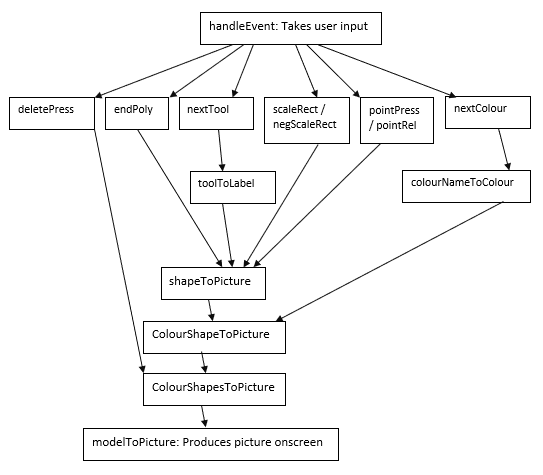
\includegraphics[width=0.85\textwidth]{program.png}
\caption{Function dependency graph - Arrows show direction of function calls}
\end{figure}

%~~~~~~~~~~~~~~~~~~~~~~~~~~~~~~~~~~~~~~~~~~~~~~~~~~~~~~~~~~~~~~~~~~~~~~~~~~~~~~~~~~~~~~~~~~~~~~~~~~~~

\section{Testing}%How did I test the program focus on methodology and testing groups
\paragraph{Part 1} 
 composed of the functions \verb|toolToLabel| \verb|nextTool| and \verb|nextColour| was tested using the provided black-box test file under the command \verb|cabal v2-test|. It passed \verb| 1 of 1 test suites| indicating correctness. Further simple white-box tests were conducted within development calling functions with edge-case inputs in the terminal to ensure the case matching was error tolerant, eventually any such errors were deemed eliminated.
 
\paragraph{Parts 2 \& 3} 
were tested firstly by removing all errors or warnings delivered by program compilation. As the Part 3 functions are designed to call the functions in both parts 1 and 2 it was decided it would be possible to test the functionality of parts 2 and 3 just through rigorous black-box testing of program GUI response. Each shape tool was tested in as many input configurations as possible including colour. Further all key inputs were tested to ensure they produced the desired response. The program passed both testing regimes. Finally, testing concluded with some white-box tests for edge cases in inputs to check for crashes or specification violations. Firstly the delete command was tested on a blank canvas and did not have any unintended consequences. Next, various variations of capTool, the most complex tool, were tested in all four coordinate quadrants and various sizes. The tool returned the appropriate outputs for cut lines above and below the defined circle and also above and below the centre of but within the circle. Further the rectangle tool was tested that it was coded as clockwise which it was. Further, the functions in part 2 were subjected to a number of Black-Box doctests all of which passed. Consequently as no errors could be found and everything held to specifications the program can be deemed correct.
%~~~~~~~~~~~~~~~~~~~~~~~~~~~~~~~~~~~~~~~~~~~~~~~~~~~~~~~~~~~~~~~~~~~~~~~~~~~~~~~~~~~~~~~~~~~~~~~~~~
\section{Reflection}
\subsection{Technical Decisions}
Part 1 used a case statement for all three functions as they were all nessisarially injective and there was no need to use guards.
 Part 2 Whilst \verb|colourNameToColour| was  very simple case matching, \verb|shapeToPicture| is more complicated, case matching on the tool used it returns a CodeWorld \verb|Picture|. For both triangle and rectangle tools the \verb|solidPolygon| function was used to create the associated picture due to the specifications of the input not aligning well to a specific CodeWorld function. For the triangle the points used were the two given points and a third given by the function \verb|otherTriPoint| that calculated the other isosceles point. For rectangles some vector maths is used in the definition to define the two other points as a translation of the first two points of a degree dictated by the scaling factor. The specifications for producing a cap required another nested case to determine if the cutoff was below the circle or not. if it was it would just return a circle, otherwise the desired cap would be produced, necessitated by the clip window and translations used. \verb|colourShapeToPicture| applied both prior part 2 functions to return a coloured picture using the appropriate CodeWorld function. Finally it was necessary to recurse through the list of colourshapes in the \verb|colourShapesToPicture| function as the list could be of any length.
 Part 3 was a simple implementation. The main function \verb|handleEvent| cased on different inputs and would, instead of nesting cases, call appropriate helper function(s) which could case on the required part of the input to produce the desired output .  To reduce the risk of errors most helpers were guarded by wildcards.

%~~~~~~~~~~~~~~~~~~~~~~~~~~~~~~~~~~~~~~~~~~~~~~~~~~~~~~~~~~~~~~~~~~~~~~~~~~~~~~~~~~~~~~~~~~~~~~~~~~~~
\subsection{Assumptions}%Describe assumptions you have made about how a user might use the program and how this has influenced your design decisions.
A gap in specifications for \verb|handleEvent| necessitated the assumption that the function \verb|pointRel| should re-initialise the scale factor of the rectangle tool at \verb|1.0| upon the completion of a rectangle on release of cursor. This is hoped to enhance functionality when a user has used an extreme value of the scale factor and wants to quickly return to a reasonable scale factor for the next rectangle input. For \verb|colourShapesToPicture| it was assumed that in case of an empty shapes list it should return a blank canvas, thus the prespecified CodeWorld function \verb|blank| was used.
\subsection{Reflection}
Due to the simple nature of and efficacy of the program the author does see any impetus to build the program differently. Further they did not run into any notable issues during development and did not find any significant strain on their technical skills. Due to its simplicity the program is very easy to interprete and is well documented.
%~~~~~~~~~~~~~~~~~~~~~~~~~~~~~~~~~~~~~~~~~~~~~~~~~~~~~~~~~~~~~~~~~~~~~~~~~~~~~~~~~~~~~~~~~~~~~~~~~~~~


%~~~~~~~~~~~~~~~~~~~~~~~~~~~~~~~~~~~~~~~~~~~~~~~~~~~~~~~~~~~~~~~~~~~~~~~~~~~~~~~~~~~~~~~~~~~~~~~~~~~~
\end{document}